\chapter{Methods of control}

\section{Radar service}

The radar service is based on the use of surveillance system imaging with
identified aircraft in order to ensure:

\begin{itemize}
\item aircraft separation,
\item air traffic monitoring, in order to inform about route deviations,
\item radar vectoring to avoid traffic or shorten the route,
\item assistance for aircraft in distress,
\item coordination of different types of air traffic,
\end{itemize} additionally, in case of radar service in approach control
service:
\begin{itemize}
\item radar vectoring to a position, from which final instrument approach can be
conducted,
\item radar vectoring to a position, from which visual approach can be
conducted,
\item monitoring instrument approach procedures and visual approaches.
\end{itemize}

In vFIR Warszawa, the following radar separation minima are applied:

\begin{description}
\item[Horizontal separation] 5.0~NM
\item[Vertical separation]\parbox[t]{0.8\textwidth}{ below FL280: 1000~ft\\
above FL280: 2000~ft, except RVSM airspace, as defined in section
\ref{sssec:airspace:rvsm}}
\end{description}

\subsubsection{APP with surveillance capabilities}

In vFIR Warszawa, radar service is available at the following positions:
\begin{itemize}
\item APP Gdańsk,
\item APP Kraków,
\item APP Poznań.
\item APP Warszawa.
\end{itemize}

\subsubsection{Reduced lateral separation}

In following TMAs, approach may reduce lateral separation to 3~NM in 30~km
(16~NM) radius from the radar antenna:
\begin{itemize}
\item TMA Gdańsk,
\item TMA Warszawa.
\end{itemize}

\subsubsection{Wake turbulence separation}

\begin{table}[htbp] \centering
  \begin{tabular}{|M{3cm}|M{3cm}|M{3cm}|} \hline\rowcolor{vred}
\color{white}\textbf{Preceding} & \color{white}\textbf{Succeeding} &
\color{white}\textbf{Separation} \\\hline SUPER (J) & \multirow{2}{*}{HEAVY (H)}
& 5 NM \\\cline{1-1}\cline{3-3} HEAVY (H) & & 4 NM \\\hline SUPER (J) &
\multirow{2}{*}{MEDIUM (M)} & 7 NM \\\cline{1-1}\cline{3-3} HEAVY (H) & & 5 NM
\\\hline SUPER (J) & \multirow{3}{*}{LIGHT (L)} & 8 NM \\\cline{1-1}\cline{3-3}
HEAVY (H) & & 6 NM \\\cline{1-1}\cline{3-3} MEDIUM (M) & & 5 NM \\\hline
  \end{tabular}
  \caption{Wake turbulence separation}
  \label{tab:wtc_radar}
\end{table}

\subsubsection{Beginning and termination of radar service}

In order to begin radar service, aircraft must be identified.

Aircraft identification is described in ICAO Doc 4444: PANS-ATM, chapter 8,
sections 8.6.2 and 8.6.3~\cite{4444}.

There are two main types of radar identification, depending on available
equipment:

\paragraph{Primary Surveillance Radar identification:} \cite[sect.
8.6.2.4]{4444}

\begin{itemize}
\item by correlating a particular radar position indication with an aircraft
reporting its position over, or as bearing and distance from, a point displayed
on the radar map, and by ascertaining that the track of the particular radar
position is consistent with the aircraft path or reported heading;
\item by correlating an observed radar position indication with an aircraft
which is known to have just departed, provided that the identification is
established within 2 km (1 NM) from the end of the runway used. Particular care
should be taken to avoid confusion with aircraft holding over or overflying the
aerodrome, or with aircraft departing from or making a missed approach over
adjacent runways;
\item by ascertaining the aircraft heading, if circumstances require, and
following a period of track observation:
  \begin{itemize}
  \item instructing the pilot to execute one or more changes of heading of 30
degrees or more and correlating the movements of one particular radar position
indication with the aircraft's acknowledged execution of the instructions given;
or
  \item correlating the movements of a particular radar position indication with
manoeuvres currently executed by an aircraft having so reported.
  \end{itemize}
\end{itemize}

\paragraph{Secondary Surveillance Radar identification:} \cite[sect.
8.6.2.3]{4444}

\begin{itemize}
\item recognition of the aircraft identification in a radar label;
\item recognition of an assigned discrete code, the setting of which has been
verified, in a radar label;
\item direct recognition of the aircraft identification of a Mode S-equipped
aircraft in a radar label;
\item observation of compliance with an instruction to set a specific code;
\item observation of compliance with an instruction to squawk IDENT;
\end{itemize}

In any case of identification, there must be reasonable assurance that there is
no possibility of mistaking the traffic for another aircraft performing under
similar flight conditions (e.g., same area, duplicate transponder code etc.)

Crew should be informed about beginning the radar service by using the phrase
\textit{``identified''} or \textit{``radar contact''}.

Radar service termination may be conducted when:

\begin{itemize}
\item aircraft exit airspace in which radar service is provided or is trasferred
to a unit that does not provide radar service;
\item aircraft descends below Minimum Vectoring Altitude (MVA);
\item identification has been lost or there is reasonable certainty that the
identification may be lost soon (e.g.~disappearing from scope and reappearing
with a different squawk code);
\item radar contact is lost;
\item aircraft has landed.
\end{itemize}

The termination of radar service should be immediately communicated to the crew
using the phrase \textit{``radar service terminated''}, except when the aircraft
has landed.

\subsubsection{Transfer of identification}

If the aircraft has been identified by the controller/flight information service
officer within vFIR Warszawa and is transferred to another ATCO/FISO that
conducts radar service, the radar identification is transferred\dots

Transfer of identification takes place only within vFIR Warszawa, unless local
procedures or agreements state otherwise.

Thanks to transfer of identification, there is no need to identify the aircraft
again (e.g. requiring squawk code assignment for ``SQUAWK DUPE'' aircraft).

\subsubsection{Prohibited practices}

The following practices and techniques should not be used in precision area
navigation:

\begin{itemize}
\item issuing instructions to fly direct to a waypoint that has been deleted
from the aircraft systems by directing the aircraft to a point further down the
procedure;
\item issuing instructions to fly direct to a waypoint that the aircraft has
already passed;
\item issuing instruction to fly direct to a waypoint that is not a part of a
procedure, unless it is a point over which a holding is published on the
procedure chart;
\end{itemize}

Those rules may not be applied in non-standard situations, if the crew confirms
that they are able to proceed to a given waypoint. Such instruction should not
include a terminal area navigation waypoint (e.g. WA533).

\section{Radar control techniques}

\subsubsection{Separation minima}

Minimum radar separation within vFIR Warszawa is \textbf{5 NM}.

In TMA Warszawa and TMA Gdańsk, reduced separation of \textbf{3 NM} is used
within 16~NM from the antenna.

\subsubsection{SID/STAR}

Departing aircraft that are unable to follow the SID should be vectored, so that
their departure routes are as close to the published procedure as possible, or
be directed to the last point of the SID.

If the arriving crew can not execute the published STAR (due to lack of required
certification, sensor degradation) APP shall begin radar vectoring. Aircraft
should be vectored so that it's route is as close to the published procedure as
possible.

In the event of any doubt by ATC or the aircraft crew regarding the correctness
of the navigation carried out, APP shall immediately switch to radar vectoring.

If radar vectoring of arriving aircraft was started in the APP sector, if
possible, when vectoring is completed it should be directed to a point on the
STAR (in case of transfer to DIR).

APP issues STAR clearance after estabishing radio communication with the
aircraft. If a shortcut is coordinated with another controller, STAR clearance
will be issued by the ATC currently controlling the aircraft.

STAR shall not be changed during it's execution. In case of arrival runway
change while the STAR is conducted, APP should revert to radar vectoring to
final approach.

\subsubsection{Continuous Descent Approach}

Continuous Descent Approach (CDA) is a technique, in which arriving aircraft
descend:

\begin{itemize}
\item with lowest thrust possible,
\item avoiding leveling off,
\item in clean configuration (gear and flaps retracted).
\end{itemize}

CDA begins at an altitude of 7000~ft or higher (depending on traffic and
meteorological situation). In a distance of around \textbf{30 track NM} from
RWY, at \textbf{FL120} or below, APP gives the crew the planned track distance.

\begin{itemize}
\item If aircraft executes P-RNAV STAR and APP/DIR plans a ``downwind leg'',
APP/DIR informs the crew about the planned position of the ``base leg'' turn.
This information is equivalent to giving the planned track distance.
\item If radar vectoring is used, APP/DIR at aroudn 25 track NM to touchdown, at
an altitude of 7000~ft or above, informs the crew of the planned track distance
to touchdown.
\end{itemize}

APP/DIR utilizes speed control as required in such a way, that Minimum Clean
Speed (MCS) or higher is maintained until 15~NM to touchdown. Below 15 NM to
touchdown, APP/DIR may begin further speed reduction below MCS so that minimum
separation between arriving aircraft is maintained.

\subsubsection{Vectoring to final approach}

Vectoring to a shorter than standard (published) final may be done only on
crew's request or when approved by the crew. APP/DIR shall inform the crew of
the length of the final the aircraft will be vectored to.

Vectoring to intercept is used for ILS, VOR and TACAN approaches. It should not
be used in case of RNP approaches.

Vectoring shall allow interception of final approach track at an angle of around
30~\degree, not more than 45{\degree}. ILS glideslope shall be intercepted
``from below''.

Aircraft executing RNP approches should be directed to the initial approach fix
of the approach and reach prescribed altitude over that fix.

Aircraft executing VOR approaches shall intercept final approach track before
reaching Final Approach Fix (FAF), at the procedure-defined altitude.

\subsubsection{Minimum Vectoring Altitude} Aircraft shall not be vectored into
uncontrolled airspace, except in emergency, during weather avoidance or on
pilot's request.

\section{Procedural approach}
\label{sec:app:procedural}

Procedural control service is performed in airspaces, in which radar service is
not provided. Procedural control is based on crew position reports. An aircraft
shall fly in the procedural airspace in accordance with published procedures.

Vectoring is prohibited in procedural airspace.

Vertical separation in procedural airspace is \textbf{1000~ft}. Horizontal
separations are defined below.

\subsection{Longitudinal separation}

\subsubsection{Based on time}

There must be a minimum interval of \textbf{10 minutes} between two aircraft
passing over the same navigation point (\cref{fig:separation:long:10min}). In
the case when the planes are flying on the same route and the first one is
faster than the second one by at least \textbf{20 kts}, the longitudinal
separation is reduced to \textbf{5 min} (\cref{fig:separation:long:5min}). If
the velocity difference is more than \textbf{40 kts}, the separation is further
reduced to \textbf{3 min} (\cref{fig:separation:long:3min}).

\begin{figure}[htbp] \centering
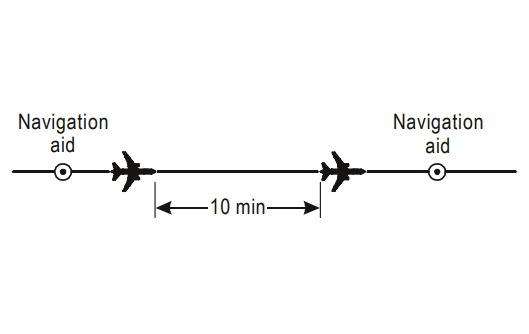
\includegraphics[width=0.5\textwidth]{4444/fig5-10.png}
  \caption{10 min separation between aircraft on same track and
level~\cite{4444}}
  \label{fig:separation:long:10min}
\end{figure}

\begin{figure}[htbp] \centering
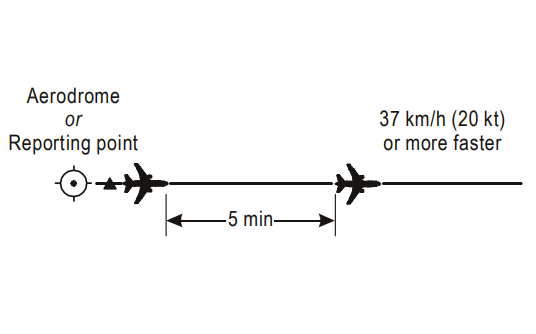
\includegraphics[width=0.5\textwidth]{4444/fig5-11.png}
  \caption{5 min separation between aircraft on same track and
level~\cite{4444}}
  \label{fig:separation:long:5min}
\end{figure}

\begin{figure}[htbp] \centering
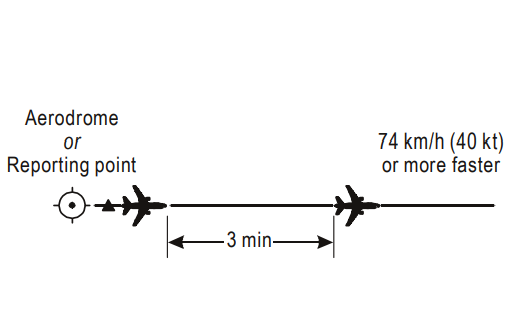
\includegraphics[width=0.5\textwidth]{4444/fig5-12.png}
  \caption{3 min separation between aircraft on same track and
level~\cite{4444}}
  \label{fig:separation:long:3min}
\end{figure}

\subsubsection{Based on DME distance}

Difference of distances reported by aircraft on same track shall be not lower
than \textbf{20 NM} (\cref{fig:separation:long:dme20}). The separation can be
reduced to \textbf{10 NM}, if the preceding aircraft is faster by at least
\textbf{20 kts} (\cref{fig:separation:long:dme10}).

\begin{figure}[htbp]
  \centering
  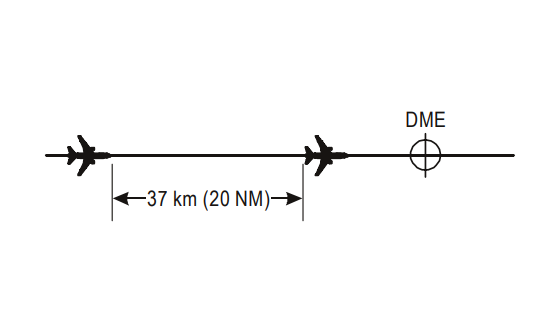
\includegraphics[width=0.5\textwidth]{4444/fig5-21.png}
  \caption{20 NM DME-based separation between aircraft on same track and
    level~\cite{4444}}
  \label{fig:separation:long:dme20}
\end{figure}

\begin{figure}[htbp]
  \centering
  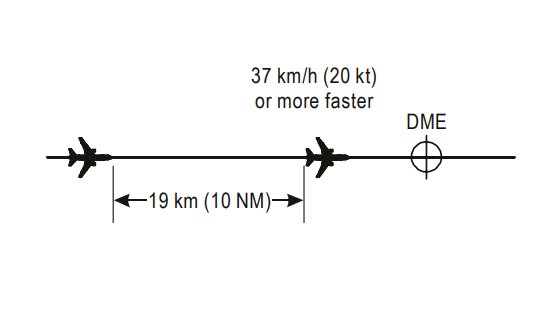
\includegraphics[width=0.5\textwidth]{4444/fig5-22.png}
  \caption{10 NM DME-based separation between aircraft on same track and
    level~\cite{4444}}
  \label{fig:separation:long:dme10}
\end{figure}

\clearpage % Remove when below section is extended
\subsection{Lateral separation}

\begin{figure}[htbp]
  \centering
  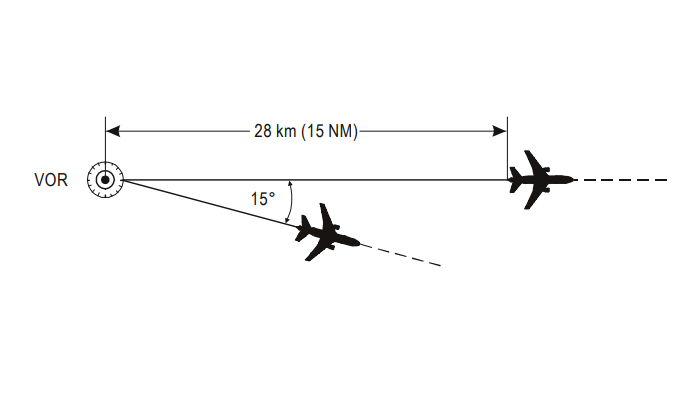
\includegraphics[width=0.5\textwidth]{4444/fig5-2.png}
  \caption{Separation using the same VOR~\cite{4444}}
  \label{fig:separation:lat:vor}
\end{figure}

\begin{figure}[htbp]
  \centering
  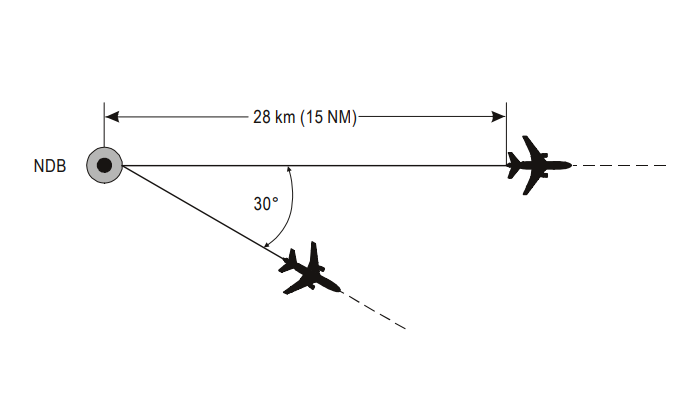
\includegraphics[width=0.5\textwidth]{4444/fig5-3.png}
  \caption{Separation using the same NDB~\cite{4444}}
  \label{fig:separation:lat:ndb}
\end{figure}

\begin{figure}[htbp]
  \centering
  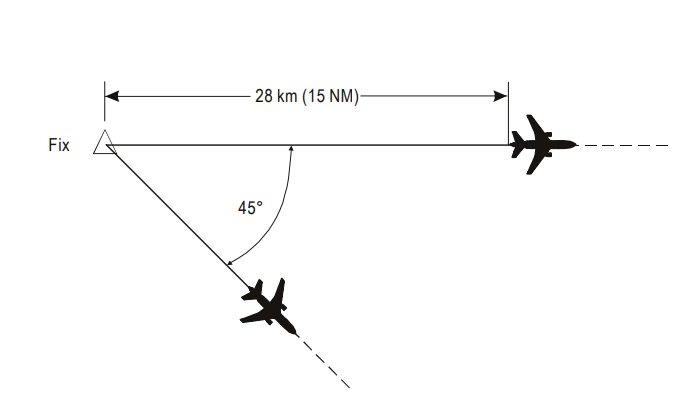
\includegraphics[width=0.5\textwidth]{4444/fig5-4.png}
  \caption{Separation using dead reckoning~\cite{4444}}
  \label{fig:separation:lat:fix}
\end{figure}

\clearpage % Remove when above section is extended
\subsection{Approach separation}

Succeeding aircraft may be cleared for approach:
\begin{itemize}
\item when the preceding aircraft is in communication with and sighted by the
  aerodrome control tower and reasonable assurance exists that a normal landing
  can be accomplished, or
\item when timed approaches are used, the preceding aircraft has passed the
  defined point inbound and reasonable assurance exists that a normal landing
  can be accomplished.
\end{itemize}

\subsection{Departure separation}
As described in \cref{sec:twr:dep}.

Other procedural separations described in Chapter 5 of ICAO Doc 4444~\cite{4444}
may be used to the extent of the controller's knowledge.

\section{Procedural control methods}
\label{sec:app:procedural_methods}

\subsubsection{Receiving position reports}

The basic tool when applying procedural control is the knowledge of aircraft's
position based on the crew's position report. The controller shall use the
reports as often as necessary in order to use appropriate techniques and methods
to maintain separation between aircraft.

\subsubsection{Information about delays}

The procedural environment is characterized by increased operation times
resulting from the need to separate traffic based on position reports. Arrivals
more frequent than once every 10 minutes can result in delays and the crews
should be informed about these delays as soon as possible.

\subsubsection{Separating departures and arrivals}

Departure separation is achieved by the use of time-based separations (see
\cref{sec:twr:dep}).

When a departure is planned it is recommended not to descend arriving aircraft
below FL110, until other separation minimum is ensured, due to departing
aircraft climbing.

If the aircraft is required to fly at FL110 for a longer period, the following
difficulties should be taken into account in returning to scheduled descent
profile at a later time.

Arriving aircraft descending while departing aircraft climb is possible. Where
vertical separation between aircraft cannot be ensured, adequate horizontal
separation must be provided. This situation is illustrated in \cref{fig:separation:climb15min}
in the example for climb, which presents a scenario divided into 3 stages:

\begin{enumerate}
\item maintained vertical separation,
\item clearance for climb --- loss of vertical separation --- horizontal
  separation must be maintaned,
\item reaching level by the climbing aircraft --- vertical separation is
  maintained again.
\end{enumerate}

\begin{figure}[htbp]
  \centering
  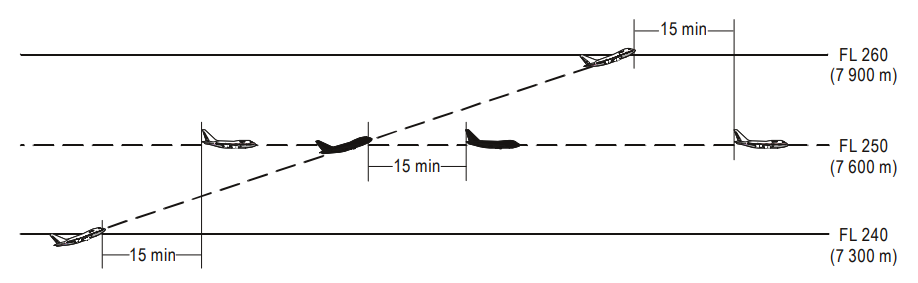
\includegraphics[width=0.5\textwidth]{4444/fig5-15A.png}
  \caption{15 min separation between aircraft climbing on the same
    track~\cite{4444}}
  \label{fig:separation:climb15min}
\end{figure}

\subsubsection{Simultaneous climb/descent of aircraft}

When aircraft on the same track are ascending/descending simultaneously, it is
recommended to use the minimum/maximum rates of climb/descent.

\subsubsection{Obtaining longitudinal time-based separation}

If the expected positions of the separated aircraft do not meet the requirements
for maintaining longitudinal separation, it is recommended to use one of the
following methods to maintain separation:
\begin{itemize}
\item utilizing vertical separation,
\item ordering the following aircraft to make an orbit to increase the distance
  from the preceeding aircraft,
\item speed control to obtain time separation
\end{itemize}

\subsubsection{Distances between points used in position reports}

ATC may use EuroScope's imaging to determine the approximate distance between
points reported by pilots during position reports.

\subsubsection{Separating opposite traffic}

In the event that two aircraft are traveling on opposite tracks, vertical
separation should be maintained for at least 10 minutes before and after the
expected time of passing (as shown in \cref{fig:separation:opposite}).

\begin{figure}[htbp]
  \centering
  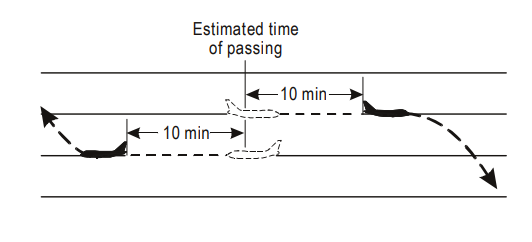
\includegraphics[width=0.5\textwidth]{4444/fig5-20.png}
  \caption{10 min separation between aircraft on reciprocal tracks~\cite{4444}}
  \label{fig:separation:opposite}
\end{figure}

\subsubsection{Useful phraseology}

\begin{description}
\item[DESCEND/CLIMB VIA STAR/SID TO (level)] clears aircraft to descend/climb to
  given level while maintaining altitude and speed restrictions defined in the
  procedure.
\item[CROSS (point) AT (level)] requires aircraft to reach certain level over
  specified position.
\item[CROSS (point) AT (level) OR ABOVE, IF UNABLE MAINTAIN (level)] as above,
  but specifies a level to maintain if reaching a given level is not possible.
\item[CROSS (point) AT (TIME) OR LATER] requires the aircraft to adjust speed in
  order to maintain time-based horizontal separation.
\item[REPORT (time/distance/radial) FROM (point)] additional, non-standard,
  position report in order to establish aircraft's postition in space.
\end{description}

\section{Silent coordination and transfer}

Transfer of control and communication shall take place in a defined standard
transfer point and level, set between sectors in this manual or a Letter of
Agreement.

If aircraft is to be transferred according to the standard rules no coordination
is required.

Coordination of shortcuts (DCT) and transfer levels (XFL) shall be done using
built-in EuroScope coordination functions.

\subsubsection{Transfer of control}

Transfer may take place no sooner than 5 minutes before reaching the Area of
Responisbility (AoR) boundary (including vertical boundaries). Transfer shall
take place at least 1 minute before the aircraft enters AoR of the next
controller.

The following transfer procedure is in use:

\begin{enumerate}
\item Issuing frequency change instruction while using the ``HAND OFF''
  function. It is interpreted as:
  \begin{itemize}
  \item transfer of radar identification,
  \item declaration of immediate tranfer of control to the receiving controller,
  \item confirmation that the aircraft is released under the conditions set in
    the ATC release.
  \end{itemize}
\item Aircraft remains ``in suspension'' until it establishes two-way radio
  communication with the next controller,
\item After establishing communications the receiving controller accepts the
  transfer by pressing ``ACCEPT''. It~is interpreted as:
  \begin{itemize}
  \item confirmation of establishing two-way communication at the designated frequency.
  \end{itemize}
\end{enumerate}

Transfer refusal (``REFUSE'') may be used only when an apparent error in next
controller selection has been made (e.g. transfer to APP Kraków instead of APP
Gdańsk). A transfer shall not be refused if there is suspicion that aircraft may
have been already transferred to incorrect frequency, even by mistake (e.g.
transfer to APP Warszawa (North) instead of APP Warszawa (South)). If the
receiving controller has used the ``REFUSE'' option, immediate contact between
controllers should be established to explain the situation.

\textbf{During transfer, the transferring controller is responsible for the separation.}

\subsubsection{Transfer conditions}

\begin{itemize}
\item Vertical separation of \textbf{1000~ft}, or
\item Lateral separation of:
  \begin{itemize}
  \item \textbf{5~NM}, when the preceding aircraft is not slower than the
    succeeding aircraft (distance constant or increasing),
  \item \textbf{10~NM}, when the preceding aircraft is slower then the
    succeeding aircraft (distance is decreasing), while ensuring that during the
    transfer of control the distance between aircraft will not decrease below 10~NM.
  \end{itemize}
\end{itemize}

\subsubsection{ATC release}

Release of control is the authority of an air traffic control unit accepting
communication to change the current flight plan before the aircraft enters its
area of responsibility. This power must be clearly delegated during
coordination, unless the local procedures or agreements between the units
concerned provides otherwise.

Transferring unit establishes the conditions of the release as a release for:
\begin{itemize}
\item climb,
\item descent,
\item change of direction,
\item change of vertical or horizontal speed.
\end{itemize}

\subsubsection{ATC release during transfer from APP to ACC and between ACC
  sectors}

Transfer of control and communication contains releases for:

\begin{itemize}
\item level change,
\item change of direction of flight,
\item change of vertical or horizontal speed.
\end{itemize}

\section{Coordination of non-standard traffic}

If the aircraft submits a non-standard request, actions should be
coordinated with all controllers that may be affected by the traffic.

%%% Local Variables:
%%% mode: latex
%%% TeX-master: "../main"
%%% End:
